% Options for packages loaded elsewhere
\PassOptionsToPackage{unicode}{hyperref}
\PassOptionsToPackage{hyphens}{url}
%
\documentclass[
]{article}
\usepackage{lmodern}
\usepackage{amsmath}
\usepackage{ifxetex,ifluatex}
\ifnum 0\ifxetex 1\fi\ifluatex 1\fi=0 % if pdftex
  \usepackage[T1]{fontenc}
  \usepackage[utf8]{inputenc}
  \usepackage{textcomp} % provide euro and other symbols
  \usepackage{amssymb}
\else % if luatex or xetex
  \usepackage{unicode-math}
  \defaultfontfeatures{Scale=MatchLowercase}
  \defaultfontfeatures[\rmfamily]{Ligatures=TeX,Scale=1}
\fi
% Use upquote if available, for straight quotes in verbatim environments
\IfFileExists{upquote.sty}{\usepackage{upquote}}{}
\IfFileExists{microtype.sty}{% use microtype if available
  \usepackage[]{microtype}
  \UseMicrotypeSet[protrusion]{basicmath} % disable protrusion for tt fonts
}{}
\makeatletter
\@ifundefined{KOMAClassName}{% if non-KOMA class
  \IfFileExists{parskip.sty}{%
    \usepackage{parskip}
  }{% else
    \setlength{\parindent}{0pt}
    \setlength{\parskip}{6pt plus 2pt minus 1pt}}
}{% if KOMA class
  \KOMAoptions{parskip=half}}
\makeatother
\usepackage{xcolor}
\IfFileExists{xurl.sty}{\usepackage{xurl}}{} % add URL line breaks if available
\IfFileExists{bookmark.sty}{\usepackage{bookmark}}{\usepackage{hyperref}}
\hypersetup{
  pdftitle={Exercise 2},
  pdfauthor={Yuting Huang, Jipeng Cheng, Weidi Hou},
  hidelinks,
  pdfcreator={LaTeX via pandoc}}
\urlstyle{same} % disable monospaced font for URLs
\usepackage[margin=1in]{geometry}
\usepackage{color}
\usepackage{fancyvrb}
\newcommand{\VerbBar}{|}
\newcommand{\VERB}{\Verb[commandchars=\\\{\}]}
\DefineVerbatimEnvironment{Highlighting}{Verbatim}{commandchars=\\\{\}}
% Add ',fontsize=\small' for more characters per line
\usepackage{framed}
\definecolor{shadecolor}{RGB}{248,248,248}
\newenvironment{Shaded}{\begin{snugshade}}{\end{snugshade}}
\newcommand{\AlertTok}[1]{\textcolor[rgb]{0.94,0.16,0.16}{#1}}
\newcommand{\AnnotationTok}[1]{\textcolor[rgb]{0.56,0.35,0.01}{\textbf{\textit{#1}}}}
\newcommand{\AttributeTok}[1]{\textcolor[rgb]{0.77,0.63,0.00}{#1}}
\newcommand{\BaseNTok}[1]{\textcolor[rgb]{0.00,0.00,0.81}{#1}}
\newcommand{\BuiltInTok}[1]{#1}
\newcommand{\CharTok}[1]{\textcolor[rgb]{0.31,0.60,0.02}{#1}}
\newcommand{\CommentTok}[1]{\textcolor[rgb]{0.56,0.35,0.01}{\textit{#1}}}
\newcommand{\CommentVarTok}[1]{\textcolor[rgb]{0.56,0.35,0.01}{\textbf{\textit{#1}}}}
\newcommand{\ConstantTok}[1]{\textcolor[rgb]{0.00,0.00,0.00}{#1}}
\newcommand{\ControlFlowTok}[1]{\textcolor[rgb]{0.13,0.29,0.53}{\textbf{#1}}}
\newcommand{\DataTypeTok}[1]{\textcolor[rgb]{0.13,0.29,0.53}{#1}}
\newcommand{\DecValTok}[1]{\textcolor[rgb]{0.00,0.00,0.81}{#1}}
\newcommand{\DocumentationTok}[1]{\textcolor[rgb]{0.56,0.35,0.01}{\textbf{\textit{#1}}}}
\newcommand{\ErrorTok}[1]{\textcolor[rgb]{0.64,0.00,0.00}{\textbf{#1}}}
\newcommand{\ExtensionTok}[1]{#1}
\newcommand{\FloatTok}[1]{\textcolor[rgb]{0.00,0.00,0.81}{#1}}
\newcommand{\FunctionTok}[1]{\textcolor[rgb]{0.00,0.00,0.00}{#1}}
\newcommand{\ImportTok}[1]{#1}
\newcommand{\InformationTok}[1]{\textcolor[rgb]{0.56,0.35,0.01}{\textbf{\textit{#1}}}}
\newcommand{\KeywordTok}[1]{\textcolor[rgb]{0.13,0.29,0.53}{\textbf{#1}}}
\newcommand{\NormalTok}[1]{#1}
\newcommand{\OperatorTok}[1]{\textcolor[rgb]{0.81,0.36,0.00}{\textbf{#1}}}
\newcommand{\OtherTok}[1]{\textcolor[rgb]{0.56,0.35,0.01}{#1}}
\newcommand{\PreprocessorTok}[1]{\textcolor[rgb]{0.56,0.35,0.01}{\textit{#1}}}
\newcommand{\RegionMarkerTok}[1]{#1}
\newcommand{\SpecialCharTok}[1]{\textcolor[rgb]{0.00,0.00,0.00}{#1}}
\newcommand{\SpecialStringTok}[1]{\textcolor[rgb]{0.31,0.60,0.02}{#1}}
\newcommand{\StringTok}[1]{\textcolor[rgb]{0.31,0.60,0.02}{#1}}
\newcommand{\VariableTok}[1]{\textcolor[rgb]{0.00,0.00,0.00}{#1}}
\newcommand{\VerbatimStringTok}[1]{\textcolor[rgb]{0.31,0.60,0.02}{#1}}
\newcommand{\WarningTok}[1]{\textcolor[rgb]{0.56,0.35,0.01}{\textbf{\textit{#1}}}}
\usepackage{graphicx}
\makeatletter
\def\maxwidth{\ifdim\Gin@nat@width>\linewidth\linewidth\else\Gin@nat@width\fi}
\def\maxheight{\ifdim\Gin@nat@height>\textheight\textheight\else\Gin@nat@height\fi}
\makeatother
% Scale images if necessary, so that they will not overflow the page
% margins by default, and it is still possible to overwrite the defaults
% using explicit options in \includegraphics[width, height, ...]{}
\setkeys{Gin}{width=\maxwidth,height=\maxheight,keepaspectratio}
% Set default figure placement to htbp
\makeatletter
\def\fps@figure{htbp}
\makeatother
\setlength{\emergencystretch}{3em} % prevent overfull lines
\providecommand{\tightlist}{%
  \setlength{\itemsep}{0pt}\setlength{\parskip}{0pt}}
\setcounter{secnumdepth}{-\maxdimen} % remove section numbering
\usepackage{booktabs}
\usepackage{longtable}
\usepackage{array}
\usepackage{multirow}
\usepackage{wrapfig}
\usepackage{float}
\usepackage{colortbl}
\usepackage{pdflscape}
\usepackage{tabu}
\usepackage{threeparttable}
\usepackage{threeparttablex}
\usepackage[normalem]{ulem}
\usepackage{makecell}
\usepackage{xcolor}
\ifluatex
  \usepackage{selnolig}  % disable illegal ligatures
\fi

\title{Exercise 2}
\author{Yuting Huang, Jipeng Cheng, Weidi Hou}
\date{3/5/2022}

\begin{document}
\maketitle

\hypertarget{problem-1-visualization}{%
\section{Problem 1: visualization}\label{problem-1-visualization}}

\hypertarget{plot-1-average-boarding-line-graph}{%
\subsection{1.1 Plot 1: average boarding line
graph}\label{plot-1-average-boarding-line-graph}}

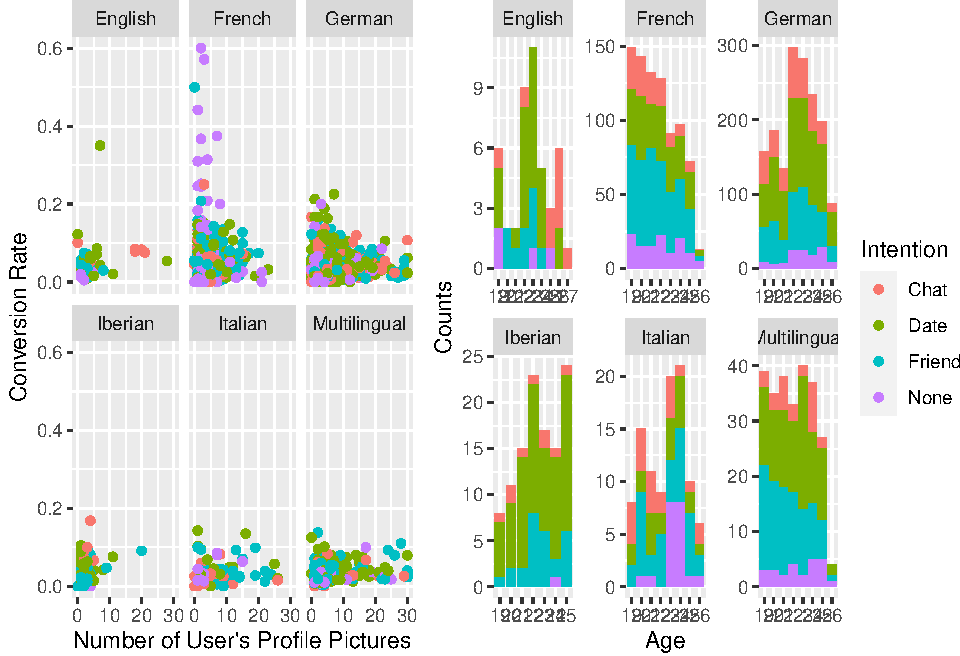
\includegraphics{Exercise2_files/figure-latex/unnamed-chunk-1-1.pdf}

According to the graph, it shows that the hour of peak boardings do not
change from day to day, and it broadly similar showing the peak hour at
15-17.

\textbf{Does the hour of peak boarding change from day to day, or is it
broadly similar across days?}

According to the graph, it shows that the hour of peak boardings do not
change from day to day, and it broadly similar showing the peak hour at
15-17.

\textbf{Why do you think average boarding on Mondays in September look
lower, compared to other days and months?}

We can guess that there are less average boardings on September because
the beginning of Fall semester. On the other hand, students may not
prefer choosing the courses on Monday due to ``Monday Blue''.

\textbf{Similarly, why do you think average boardings on Weds/Thurs/Fri
in November look lower?}

Average boarding on Weds/Thurs/Fri in November look lower because
students may have to prepare for the midterm exam, they would like to
stay home rather than go outside.

\hypertarget{plot-2-scatter-plots-showing-boardings-vs.-temperature}{%
\subsection{1.2 Plot 2: scatter plots showing boardings
vs.~temperature}\label{plot-2-scatter-plots-showing-boardings-vs.-temperature}}

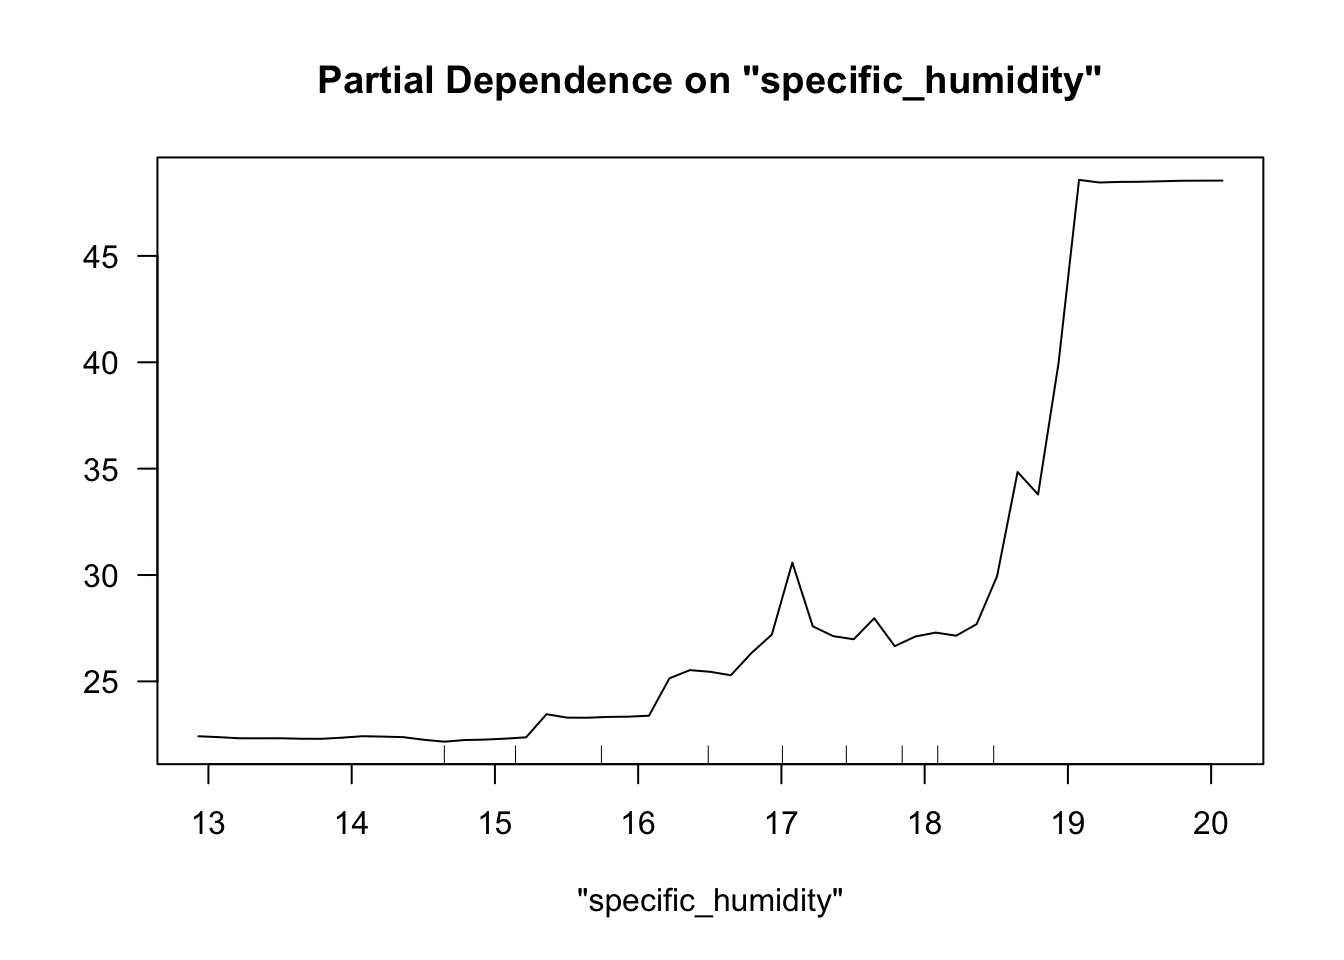
\includegraphics{Exercise2_files/figure-latex/unnamed-chunk-2-1.pdf}

\textbf{When we hold hour of day and weekend status constant, does
temperature seem to have a noticeable effect on the number of UT
students riding the bus?}

According to above graph, temperature seem to have no noticeable effect
on the number of UT students riding the bus.

\hypertarget{problem-2-saratoga-house-prices}{%
\section{Problem 2: Saratoga house
prices}\label{problem-2-saratoga-house-prices}}

\hypertarget{the-best-linear-model}{%
\subsection{2.1 The best linear model}\label{the-best-linear-model}}

\begin{verbatim}
## errs_lm1 errs_lm2 errs_lm3 errs_lm4 
## 77281.30 66551.42 70448.49 64810.81
\end{verbatim}

\textbf{Build the best linear model for price that you can. It should
clearly outperform the ``medium'' model that we considered in class. Use
any combination of transformations, engineering features, polynomial
terms, and interactions that you want; and use any strategy for
selecting the model that you want.}

The result suggests that lm4 is the best, since it has the lowest cross
validation rmse. The formular of linear model 4 is as below. The
cross-validation rmse of lm4 is smaller than that of medium model.
Therefore, our model overperfom the medium model.

\$price=livingarea+centralair+bathrooms+fuel+lotsize+bedrooms+rooms+livingarea\times centralair+livingarea
\times bathrooms+livingarea \times fuel+livingarea
\times rooms+bathrooms \times bedrooms+centralair \times fuel+bathroom
\times fuel+fuel \times lotsize+centralair \times bathrooms+bedrooms
\times rooms \$

\hypertarget{the-best-knn}{%
\subsection{2.2 The Best KNN}\label{the-best-knn}}

We will find optimal k and features simultaneously.

\begin{verbatim}
##       k      err  std_err
## knn1 46 77680.84 1650.026
## knn2 19 68336.87 1892.960
## knn3 28 68963.82 1659.971
\end{verbatim}

\textbf{Which model seems to do better at achieving lower out-of-sample
mean-squared error?}

Analysis: According to our results, the cross-validation error is lower
for linear model, so linear model seems to do better at achieving lower
out of sample mean squared error. However, the best variables and
cross-validation error for knn and linear model is pretty similar, the
difference is \(68217.62-64837.09=3380.53\), which is very small
compared to their value.

\hypertarget{problem-3-classification-and-retrospective-sampling}{%
\section{problem 3: Classification and retrospective
sampling}\label{problem-3-classification-and-retrospective-sampling}}

\hypertarget{bar-plot-of-default-probability-by-credit-history}{%
\subsection{3.1 bar plot of default probability by credit
history}\label{bar-plot-of-default-probability-by-credit-history}}

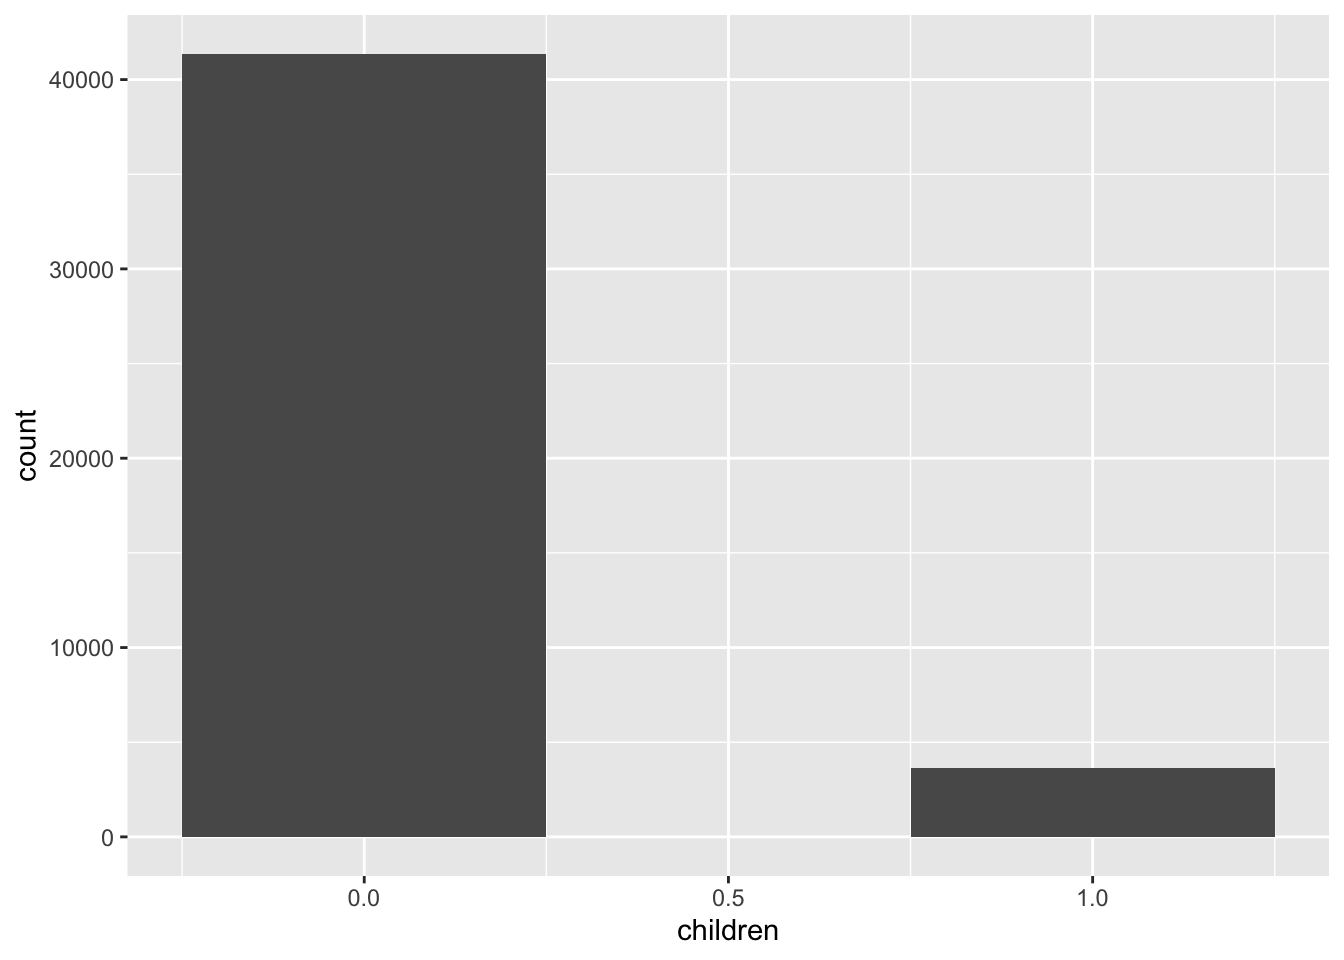
\includegraphics{Exercise2_files/figure-latex/unnamed-chunk-5-1.pdf}

\hypertarget{logistic-regression-model}{%
\subsection{3.2 logistic regression
model}\label{logistic-regression-model}}

\begin{Shaded}
\begin{Highlighting}[]
\NormalTok{g\_c\_glm }\OtherTok{=} \FunctionTok{glm}\NormalTok{(}\AttributeTok{formula =}\NormalTok{ Default }\SpecialCharTok{\textasciitilde{}}\NormalTok{ duration }\SpecialCharTok{+}\NormalTok{ amount }\SpecialCharTok{+}\NormalTok{ installment }\SpecialCharTok{+}\NormalTok{ age }\SpecialCharTok{+} 
\NormalTok{      history }\SpecialCharTok{+}\NormalTok{ purpose }\SpecialCharTok{+}\NormalTok{ foreign, }\AttributeTok{family =} \StringTok{"binomial"}\NormalTok{, }\AttributeTok{data =}\NormalTok{ g\_c)}
\end{Highlighting}
\end{Shaded}

\textbf{What do you notice about the history variable vis-a-vis
predicting defaults? What do you think is going on here? In light of
what you see here, do you think this data set is appropriate for
building a predictive model of defaults, if the purpose of the model is
to screen prospective borrowers to classify them into ``high'' versus
``low'' probability of default? Why or why not---and if not, would you
recommend any changes to the bank's sampling scheme?}

Based on the data, the default probability of people with good history
is higher than the default probability of people with poor history.
There is a sampling problem in this model, since this model based on the
``case-control'' design. To be specific, if we want to choose three
features as factors in the model, but only two of them have been chosen
in to the model but one feature has been omitted, it will lead to more
incorrect analysis for those two features. It's a type of problem of
selection bias and misrepresentation. Based on our previous analysis,
this data set is inappropriate for building a predictive model of
defaults. We recommend the bank change their sampling scheme in order to
solve the unbalanced sample problem, such as using random sampling
method.

\hypertarget{problem-4-children-and-hotel-reservations}{%
\section{problem 4: Children and hotel
reservations}\label{problem-4-children-and-hotel-reservations}}

\hypertarget{build-model}{%
\subsection{4.1 build model}\label{build-model}}

Count the dependent variable:
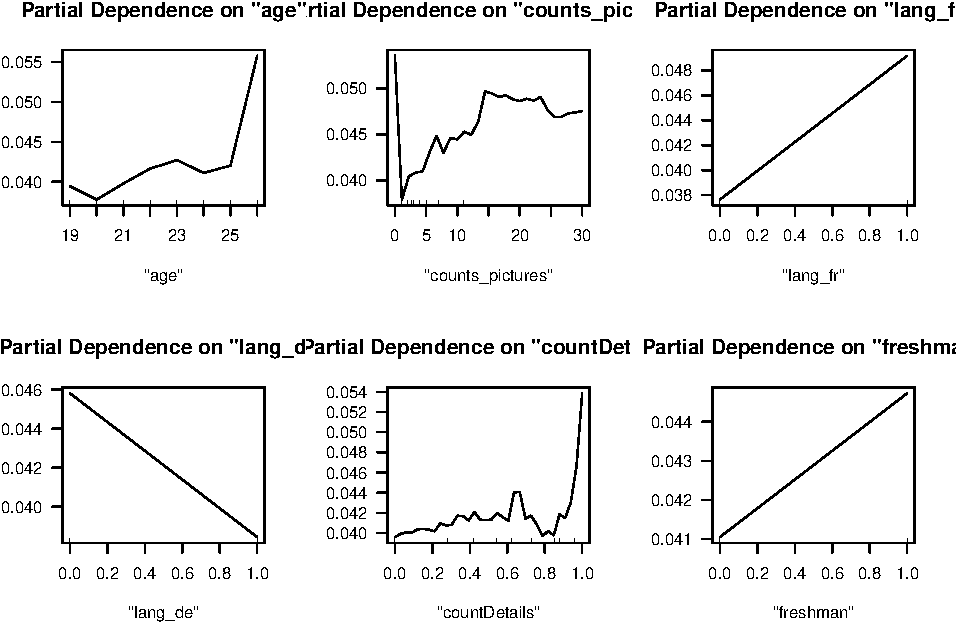
\includegraphics{Exercise2_files/figure-latex/unnamed-chunk-7-1.pdf}

\hypertarget{build-baseline-model}{%
\subsubsection{4.1.1 Build baseline model}\label{build-baseline-model}}

\begin{Shaded}
\begin{Highlighting}[]
\NormalTok{baseline1 }\OtherTok{=} \FunctionTok{glm}\NormalTok{(children }\SpecialCharTok{\textasciitilde{}}\NormalTok{ market\_segment }\SpecialCharTok{+}\NormalTok{ adults }\SpecialCharTok{+}\NormalTok{ customer\_type }\SpecialCharTok{+}\NormalTok{ is\_repeated\_guest,}
                \AttributeTok{data =}\NormalTok{ hotel\_dev\_train, }\AttributeTok{family =} \StringTok{"binomial"}\NormalTok{)}
\NormalTok{baseline2 }\OtherTok{=} \FunctionTok{glm}\NormalTok{(children }\SpecialCharTok{\textasciitilde{}}\NormalTok{ . }\SpecialCharTok{{-}}\NormalTok{ arrival\_date , }\AttributeTok{data =}\NormalTok{ hotel\_dev\_train, }\AttributeTok{family =} \StringTok{"binomial"}\NormalTok{)}
\end{Highlighting}
\end{Shaded}

\hypertarget{build-best-model---feature-engineering-with-lasso}{%
\subsubsection{4.2 Build best model - Feature engineering with
LASSO}\label{build-best-model---feature-engineering-with-lasso}}

idea: use LASSO to find main effects + interaction by eyeballing

\begin{Shaded}
\begin{Highlighting}[]
\NormalTok{hotel\_lasso\_x\_main }\OtherTok{=} \FunctionTok{model.matrix}\NormalTok{(children }\SpecialCharTok{\textasciitilde{}}\NormalTok{  (.}\SpecialCharTok{{-}}\DecValTok{1}\SpecialCharTok{{-}}\NormalTok{arrival\_date), }\AttributeTok{data=}\NormalTok{hotel\_dev\_train)}
\NormalTok{hotel\_lasso\_x\_itac }\OtherTok{=} \FunctionTok{model.matrix}\NormalTok{(children }\SpecialCharTok{\textasciitilde{}}\NormalTok{  (.}\SpecialCharTok{{-}}\DecValTok{1}\SpecialCharTok{{-}}\NormalTok{arrival\_date)}\SpecialCharTok{\^{}}\DecValTok{2}\NormalTok{, }\AttributeTok{data=}\NormalTok{hotel\_dev\_train)}
\NormalTok{hotel\_lasso\_y }\OtherTok{=}\NormalTok{ hotel\_dev\_train}\SpecialCharTok{$}\NormalTok{children}
\CommentTok{\#//see https://cran.r{-}project.org/web/packages/gamlr/gamlr.pdf to see more}
\NormalTok{hotel\_lasso\_main }\OtherTok{=} \FunctionTok{cv.gamlr}\NormalTok{(hotel\_lasso\_x\_main, hotel\_lasso\_y, }\AttributeTok{nfold=}\DecValTok{10}\NormalTok{, }\AttributeTok{verb=}\ConstantTok{TRUE}\NormalTok{, }\AttributeTok{family=}\StringTok{"binomial"}\NormalTok{)}
\end{Highlighting}
\end{Shaded}

\begin{verbatim}
## fold 1,2,3,4,5,6,7,8,9,10,done.
\end{verbatim}

\begin{Shaded}
\begin{Highlighting}[]
\NormalTok{hotel\_lasso\_itac }\OtherTok{=} \FunctionTok{cv.gamlr}\NormalTok{(hotel\_lasso\_x\_itac, hotel\_lasso\_y, }\AttributeTok{nfold=}\DecValTok{10}\NormalTok{, }\AttributeTok{verb=}\ConstantTok{TRUE}\NormalTok{, }\AttributeTok{family=}\StringTok{"binomial"}\NormalTok{)}
\end{Highlighting}
\end{Shaded}

\begin{verbatim}
## fold 1,2,3,4,5,6,7,8,9,10,done.
\end{verbatim}

\textbf{Extract strong single covariates:}

\begin{verbatim}
## 49 x 1 sparse Matrix of class "dgCMatrix"
##                                           seg100
## intercept                          -4.3116762105
## hotelCity_Hotel                     0.6896335094
## hotelResort_Hotel                  -0.0009319158
## lead_time                           0.0004653027
## stays_in_weekend_nights             0.0375017585
## stays_in_week_nights               -0.0095641930
## adults                             -0.5032745346
## mealFB                              0.7010368514
## mealHB                              0.0038399413
## mealSC                             -1.0943902454
## mealUndefined                       .           
## market_segmentComplementary         0.0709477690
## market_segmentCorporate            -1.0691813832
## market_segmentDirect                .           
## market_segmentGroups               -1.1155211678
## market_segmentOffline_TA/TO         .           
## market_segmentOnline_TA             0.0633612096
## distribution_channelDirect          0.1300222909
## distribution_channelGDS            -1.4167476886
## distribution_channelTA/TO           .           
## is_repeated_guest                  -0.8511543139
## previous_cancellations              .           
## previous_bookings_not_canceled     -0.1068481918
## reserved_room_typeB                 1.5609662780
## reserved_room_typeC                 2.7964059301
## reserved_room_typeD                -0.8687047481
## reserved_room_typeE                 .           
## reserved_room_typeF                 1.6865860121
## reserved_room_typeG                 2.3631478631
## reserved_room_typeH                 2.9595742391
## assigned_room_typeB                 0.3135503175
## assigned_room_typeC                 1.4935973872
## assigned_room_typeD                 0.9011909925
## assigned_room_typeE                 0.5490721995
## assigned_room_typeF                 0.7957113071
## assigned_room_typeG                 1.0110978443
## assigned_room_typeH                 1.4389009609
## assigned_room_typeI                 1.0519857083
## assigned_room_typeK                 .           
## booking_changes                     0.2261390737
## deposit_typeNon_Refund              .           
## deposit_typeRefundable              .           
## days_in_waiting_list               -0.0013132655
## customer_typeGroup                  .           
## customer_typeTransient              0.2359595319
## customer_typeTransient-Party       -0.4886175708
## average_daily_rate                  0.0099195983
## required_car_parking_spacesparking  0.0037021341
## total_of_special_requests           0.4736335163
\end{verbatim}

From the output, we see that the variable \textbf{deposit\_type} is
insignificant from zero. Therefore, we rule out it.

\textbf{Extract strong interactions:}

\begin{verbatim}
##                            strong_interaction_name strong_interaction_beta
## 1      market_segmentOnline_TA:reserved_room_typeB       -3.50389285799462
## 2  market_segmentOffline_TA/TO:reserved_room_typeH        3.47885225813192
## 3            hotelResort_Hotel:reserved_room_typeB        3.26317651092536
## 4                       mealHB:reserved_room_typeF        3.05422571817688
## 5  market_segmentComplementary:reserved_room_typeC        2.96741930146009
## 6                mealUndefined:assigned_room_typeD       -2.88145247830629
## 7          reserved_room_typeB:assigned_room_typeI        2.87217841953396
## 8          reserved_room_typeG:assigned_room_typeG        2.83807895321379
## 9                              reserved_room_typeE        2.79073272157387
## 10                             reserved_room_typeF        2.63805465937019
## 11               mealUndefined:assigned_room_typeB        -2.6175574095838
## 12         reserved_room_typeB:assigned_room_typeG        2.60877581914077
## 13         reserved_room_typeH:assigned_room_typeF        2.54127908608454
## 14               mealUndefined:reserved_room_typeG       -2.51347516664378
## 15         reserved_room_typeB:assigned_room_typeB       -2.45744922440907
## 16           hotelResort_Hotel:reserved_room_typeE       -2.43111864289319
## 17     market_segmentOnline_TA:reserved_room_typeD        2.39838354186488
## 18                      mealSC:reserved_room_typeG        2.33443704732597
## 19 market_segmentComplementary:reserved_room_typeF        2.32359262227225
## 20      reserved_room_typeB:deposit_typeRefundable       -2.31249556974952
## 21         reserved_room_typeD:assigned_room_typeB        2.23810494788663
## 22                             reserved_room_typeG        2.17693044547545
## 23                      mealFB:assigned_room_typeK        2.17058856221184
## 24                      mealSC:reserved_room_typeF       -2.13544346049765
## 25        market_segmentGroups:assigned_room_typeH         2.0712361525871
## 26         reserved_room_typeB:assigned_room_typeF         1.9714977208534
## 27           adults:previous_bookings_not_canceled       -1.87842854457828
## 28               mealUndefined:reserved_room_typeE        -1.7298273339858
## 29         reserved_room_typeF:assigned_room_typeK        1.65566912617863
## 30         reserved_room_typeD:assigned_room_typeC        1.53928515673223
##    abs_beta
## 1  3.503893
## 2  3.478852
## 3  3.263177
## 4  3.054226
## 5  2.967419
## 6  2.881452
## 7  2.872178
## 8  2.838079
## 9  2.790733
## 10 2.638055
## 11 2.617557
## 12 2.608776
## 13 2.541279
## 14 2.513475
## 15 2.457449
## 16 2.431119
## 17 2.398384
## 18 2.334437
## 19 2.323593
## 20 2.312496
## 21 2.238105
## 22 2.176930
## 23 2.170589
## 24 2.135443
## 25 2.071236
## 26 1.971498
## 27 1.878429
## 28 1.729827
## 29 1.655669
## 30 1.539285
\end{verbatim}

From the results, we pick these terms:
\(meal \times \text{reserved_room_type}\),
\(\text{assigned_room_type} \times \text{reserved_room_type}\),
\(hotel \times \text{reserved_room_type}\),
\(\text{market_segment} \times \text{reserved_room_type}\),\(meal \times \text{is_repeated_guest}\),
\(adult \times \text{previous_bookings_not_canceled}\),
\(meal \times \text{previous_bookings_not_canceled}\),
\(\text{market_segment}\times \times \text{customer_type}\),
\(\text{is_repeated_guest} \times \text{assigned_room_type}\),
\(\text{assigned_room_type} \times \text{required_car_parking_spaces}\)
by eyeballing, since they are significant from zero.

\textbf{Rule out non-converged covariates \& interactions:}

\begin{verbatim}
##                                              (Intercept) 
##                                            -1.342126e+01 
##                                        hotelResort_Hotel 
##                                            -7.985168e-01 
##                                                lead_time 
##                                             1.309757e-03 
##                                  stays_in_weekend_nights 
##                                             7.615960e-02 
##                                     stays_in_week_nights 
##                                            -3.597046e-02 
##                                                   adults 
##                                            -6.744400e-01 
##                                                   mealFB 
##                                             1.575158e+00 
##                                                   mealHB 
##                                             2.766487e-01 
##                                                   mealSC 
##                                            -1.420560e+00 
##                                            mealUndefined 
##                                             7.245373e-01 
##                              market_segmentComplementary 
##                                             3.987454e+01 
##                                  market_segmentCorporate 
##                                            -1.250233e+01 
##                                     market_segmentDirect 
##                                             1.231303e+01 
##                                     market_segmentGroups 
##                                            -1.612067e+01 
##                              market_segmentOffline_TA/TO 
##                                             1.055497e+01 
##                                  market_segmentOnline_TA 
##                                             9.727434e+00 
##                               distribution_channelDirect 
##                                             2.760373e-01 
##                                  distribution_channelGDS 
##                                            -2.075443e+01 
##                                distribution_channelTA/TO 
##                                            -6.067538e-01 
##                                        is_repeated_guest 
##                                             3.900822e-01 
##                                   previous_cancellations 
##                                            -1.345370e-01 
##                           previous_bookings_not_canceled 
##                                            -1.262988e+00 
##                                      reserved_room_typeB 
##                                             1.721796e+00 
##                                      reserved_room_typeC 
##                                            -5.262099e+01 
##                                      reserved_room_typeD 
##                                            -1.300977e-01 
##                                      reserved_room_typeE 
##                                            -2.468498e+00 
##                                      reserved_room_typeF 
##                                             4.478703e+00 
##                                      reserved_room_typeG 
##                                            -2.440892e+01 
##                                      reserved_room_typeH 
##                                            -2.542306e+13 
##                                      assigned_room_typeB 
##                                             7.113921e-01 
##                                      assigned_room_typeC 
##                                             1.749178e+00 
##                                      assigned_room_typeD 
##                                             1.329879e+00 
##                                      assigned_room_typeE 
##                                             8.869693e-01 
##                                      assigned_room_typeF 
##                                             9.661210e-01 
##                                      assigned_room_typeG 
##                                             5.243897e-01 
##                                      assigned_room_typeH 
##                                             1.551034e+00 
##                                      assigned_room_typeI 
##                                            -7.870813e-02 
##                                      assigned_room_typeK 
##                                            -2.161774e-01 
##                                          booking_changes 
##                                             2.336411e-01 
##                                     days_in_waiting_list 
##                                            -1.718376e-04 
##                                       customer_typeGroup 
##                                             1.214496e+00 
##                                   customer_typeTransient 
##                                             1.428212e+00 
##                             customer_typeTransient-Party 
##                                             8.247292e-01 
##                                       average_daily_rate 
##                                             1.049398e-02 
##                       required_car_parking_spacesparking 
##                                             4.864140e-01 
##                                total_of_special_requests 
##                                             5.284952e-01 
##                               mealFB:reserved_room_typeB 
##                                                       NA 
##                               mealHB:reserved_room_typeB 
##                                            -1.120220e+00 
##                               mealSC:reserved_room_typeB 
##                                             7.839458e-01 
##                        mealUndefined:reserved_room_typeB 
##                                                       NA 
##                               mealFB:reserved_room_typeC 
##                                            -3.807476e+00 
##                               mealHB:reserved_room_typeC 
##                                            -4.780170e-02 
##                               mealSC:reserved_room_typeC 
##                                             2.757082e+01 
##                        mealUndefined:reserved_room_typeC 
##                                            -2.696556e+00 
##                               mealFB:reserved_room_typeD 
##                                            -3.376330e-01 
##                               mealHB:reserved_room_typeD 
##                                            -2.341544e-01 
##                               mealSC:reserved_room_typeD 
##                                             1.924837e+00 
##                        mealUndefined:reserved_room_typeD 
##                                             2.591211e-01 
##                               mealFB:reserved_room_typeE 
##                                            -2.565681e+01 
##                               mealHB:reserved_room_typeE 
##                                            -2.051940e-01 
##                               mealSC:reserved_room_typeE 
##                                            -4.638108e+01 
##                        mealUndefined:reserved_room_typeE 
##                                             3.259557e-01 
##                               mealFB:reserved_room_typeF 
##                                            -2.594605e+01 
##                               mealHB:reserved_room_typeF 
##                                            -4.024486e-01 
##                               mealSC:reserved_room_typeF 
##                                             3.225226e+00 
##                        mealUndefined:reserved_room_typeF 
##                                            -2.623232e+01 
##                               mealFB:reserved_room_typeG 
##                                             2.529551e+01 
##                               mealHB:reserved_room_typeG 
##                                            -2.928269e-01 
##                               mealSC:reserved_room_typeG 
##                                            -4.710488e+01 
##                        mealUndefined:reserved_room_typeG 
##                                             2.672762e+01 
##                               mealFB:reserved_room_typeH 
##                                            -2.757445e+01 
##                               mealHB:reserved_room_typeH 
##                                            -6.625969e-02 
##                               mealSC:reserved_room_typeH 
##                                                       NA 
##                        mealUndefined:reserved_room_typeH 
##                                                       NA 
##                  reserved_room_typeB:assigned_room_typeB 
##                                            -6.861040e-01 
##                  reserved_room_typeC:assigned_room_typeB 
##                                             2.659826e-02 
##                  reserved_room_typeD:assigned_room_typeB 
##                                             2.939172e-01 
##                  reserved_room_typeE:assigned_room_typeB 
##                                             2.449860e+01 
##                  reserved_room_typeF:assigned_room_typeB 
##                                            -3.724704e+00 
##                  reserved_room_typeG:assigned_room_typeB 
##                                             5.110584e+01 
##                  reserved_room_typeH:assigned_room_typeB 
##                                                       NA 
##                  reserved_room_typeB:assigned_room_typeC 
##                                                       NA 
##                  reserved_room_typeC:assigned_room_typeC 
##                                             2.671289e+01 
##                  reserved_room_typeD:assigned_room_typeC 
##                                             5.750819e-01 
##                  reserved_room_typeE:assigned_room_typeC 
##                                             1.700121e+01 
##                  reserved_room_typeF:assigned_room_typeC 
##                                                       NA 
##                  reserved_room_typeG:assigned_room_typeC 
##                                                       NA 
##                  reserved_room_typeH:assigned_room_typeC 
##                                                       NA 
##                  reserved_room_typeB:assigned_room_typeD 
##                                            -5.523295e-01 
##                  reserved_room_typeC:assigned_room_typeD 
##                                             2.598090e+01 
##                  reserved_room_typeD:assigned_room_typeD 
##                                            -1.071972e+00 
##                  reserved_room_typeE:assigned_room_typeD 
##                                            -2.630963e+01 
##                  reserved_room_typeF:assigned_room_typeD 
##                                                       NA 
##                  reserved_room_typeG:assigned_room_typeD 
##                                                       NA 
##                  reserved_room_typeH:assigned_room_typeD 
##                                             2.542306e+13 
##                  reserved_room_typeB:assigned_room_typeE 
##                                            -2.518048e+01 
##                  reserved_room_typeC:assigned_room_typeE 
##                                             2.774253e+01 
##                  reserved_room_typeD:assigned_room_typeE 
##                                            -6.367419e-01 
##                  reserved_room_typeE:assigned_room_typeE 
##                                            -1.320366e+00 
##                  reserved_room_typeF:assigned_room_typeE 
##                                            -1.915089e+00 
##                  reserved_room_typeG:assigned_room_typeE 
##                                             5.329485e+01 
##                  reserved_room_typeH:assigned_room_typeE 
##                                                       NA 
##                  reserved_room_typeB:assigned_room_typeF 
##                                             2.458398e+01 
##                  reserved_room_typeC:assigned_room_typeF 
##                                             5.326504e+01 
##                  reserved_room_typeD:assigned_room_typeF 
##                                            -4.557406e-01 
##                  reserved_room_typeE:assigned_room_typeF 
##                                            -1.226703e+00 
##                  reserved_room_typeF:assigned_room_typeF 
##                                            -1.455324e+00 
##                  reserved_room_typeG:assigned_room_typeF 
##                                             2.660289e+01 
##                  reserved_room_typeH:assigned_room_typeF 
##                                                       NA 
##                  reserved_room_typeB:assigned_room_typeG 
##                                             2.187549e+00 
##                  reserved_room_typeC:assigned_room_typeG 
##                                             5.286725e+01 
##                  reserved_room_typeD:assigned_room_typeG 
##                                             3.496237e-01 
##                  reserved_room_typeE:assigned_room_typeG 
##                                            -1.819071e+00 
##                  reserved_room_typeF:assigned_room_typeG 
##                                            -2.953299e-01 
##                  reserved_room_typeG:assigned_room_typeG 
##                                             2.650580e+01 
##                  reserved_room_typeH:assigned_room_typeG 
##                                             2.542306e+13 
##                  reserved_room_typeB:assigned_room_typeH 
##                                                       NA 
##                  reserved_room_typeC:assigned_room_typeH 
##                                             2.765389e+01 
##                  reserved_room_typeD:assigned_room_typeH 
##                                            -7.330745e-01 
##                  reserved_room_typeE:assigned_room_typeH 
##                                            -2.662309e+01 
##                  reserved_room_typeF:assigned_room_typeH 
##                                            -2.211726e+01 
##                  reserved_room_typeG:assigned_room_typeH 
##                                             2.483153e+01 
##                  reserved_room_typeH:assigned_room_typeH 
##                                             2.542306e+13 
##                  reserved_room_typeB:assigned_room_typeI 
##                                                       NA 
##                  reserved_room_typeC:assigned_room_typeI 
##                                             5.175937e+01 
##                  reserved_room_typeD:assigned_room_typeI 
##                                             1.384531e+00 
##                  reserved_room_typeE:assigned_room_typeI 
##                                            -2.143034e+01 
##                  reserved_room_typeF:assigned_room_typeI 
##                                            -1.889424e-01 
##                  reserved_room_typeG:assigned_room_typeI 
##                                             2.766115e+01 
##                  reserved_room_typeH:assigned_room_typeI 
##                                             2.542306e+13 
##                  reserved_room_typeB:assigned_room_typeK 
##                                            -2.509474e+01 
##                  reserved_room_typeC:assigned_room_typeK 
##                                                       NA 
##                  reserved_room_typeD:assigned_room_typeK 
##                                            -2.379284e+01 
##                  reserved_room_typeE:assigned_room_typeK 
##                                            -2.548376e+01 
##                  reserved_room_typeF:assigned_room_typeK 
##                                            -2.140270e+00 
##                  reserved_room_typeG:assigned_room_typeK 
##                                             5.163910e+01 
##                  reserved_room_typeH:assigned_room_typeK 
##                                                       NA 
##                    hotelResort_Hotel:reserved_room_typeB 
##                                            -2.351554e+01 
##                    hotelResort_Hotel:reserved_room_typeC 
##                                             2.845077e+01 
##                    hotelResort_Hotel:reserved_room_typeD 
##                                             6.745517e-01 
##                    hotelResort_Hotel:reserved_room_typeE 
##                                            -9.015007e-01 
##                    hotelResort_Hotel:reserved_room_typeF 
##                                            -2.886894e+00 
##                    hotelResort_Hotel:reserved_room_typeG 
##                                             1.411625e+00 
##                    hotelResort_Hotel:reserved_room_typeH 
##                                                       NA 
##          market_segmentComplementary:reserved_room_typeB 
##                                             1.285741e+00 
##              market_segmentCorporate:reserved_room_typeB 
##                                             2.452451e+00 
##                 market_segmentDirect:reserved_room_typeB 
##                                            -9.225295e-02 
##                 market_segmentGroups:reserved_room_typeB 
##                                             2.776284e+00 
##          market_segmentOffline_TA/TO:reserved_room_typeB 
##                                             2.690929e-01 
##              market_segmentOnline_TA:reserved_room_typeB 
##                                                       NA 
##          market_segmentComplementary:reserved_room_typeC 
##                                            -2.593074e+01 
##              market_segmentCorporate:reserved_room_typeC 
##                                             4.289042e+00 
##                 market_segmentDirect:reserved_room_typeC 
##                                             5.933732e-01 
##                 market_segmentGroups:reserved_room_typeC 
##                                             3.095372e+00 
##          market_segmentOffline_TA/TO:reserved_room_typeC 
##                                             6.450155e-01 
##              market_segmentOnline_TA:reserved_room_typeC 
##                                                       NA 
##          market_segmentComplementary:reserved_room_typeD 
##                                             7.365686e-01 
##              market_segmentCorporate:reserved_room_typeD 
##                                             6.571157e-01 
##                 market_segmentDirect:reserved_room_typeD 
##                                             3.598426e-01 
##                 market_segmentGroups:reserved_room_typeD 
##                                             2.126027e-01 
##          market_segmentOffline_TA/TO:reserved_room_typeD 
##                                             2.594300e-01 
##              market_segmentOnline_TA:reserved_room_typeD 
##                                            -6.681195e-01 
##          market_segmentComplementary:reserved_room_typeE 
##                                             6.294372e+00 
##              market_segmentCorporate:reserved_room_typeE 
##                                            -1.800913e+01 
##                 market_segmentDirect:reserved_room_typeE 
##                                             4.817394e+00 
##                 market_segmentGroups:reserved_room_typeE 
##                                            -2.645901e+01 
##          market_segmentOffline_TA/TO:reserved_room_typeE 
##                                             4.666780e+00 
##              market_segmentOnline_TA:reserved_room_typeE 
##                                             3.175946e+00 
##          market_segmentComplementary:reserved_room_typeF 
##                                             2.153613e-02 
##              market_segmentCorporate:reserved_room_typeF 
##                                             3.168857e+00 
##                 market_segmentDirect:reserved_room_typeF 
##                                            -6.533007e-01 
##                 market_segmentGroups:reserved_room_typeF 
##                                            -2.297970e+01 
##          market_segmentOffline_TA/TO:reserved_room_typeF 
##                                            -7.237138e-01 
##              market_segmentOnline_TA:reserved_room_typeF 
##                                                       NA 
##          market_segmentComplementary:reserved_room_typeG 
##                                            -9.842682e-01 
##              market_segmentCorporate:reserved_room_typeG 
##                                            -2.513946e+01 
##                 market_segmentDirect:reserved_room_typeG 
##                                            -3.210670e-01 
##                 market_segmentGroups:reserved_room_typeG 
##                                            -2.510406e+01 
##          market_segmentOffline_TA/TO:reserved_room_typeG 
##                                             9.279120e-01 
##              market_segmentOnline_TA:reserved_room_typeG 
##                                                       NA 
##          market_segmentComplementary:reserved_room_typeH 
##                                                       NA 
##              market_segmentCorporate:reserved_room_typeH 
##                                                       NA 
##                 market_segmentDirect:reserved_room_typeH 
##                                            -2.345049e+00 
##                 market_segmentGroups:reserved_room_typeH 
##                                                       NA 
##          market_segmentOffline_TA/TO:reserved_room_typeH 
##                                                       NA 
##              market_segmentOnline_TA:reserved_room_typeH 
##                                                       NA 
##                                 mealFB:is_repeated_guest 
##                                            -2.411654e+00 
##                                 mealHB:is_repeated_guest 
##                                             5.685270e-02 
##                                 mealSC:is_repeated_guest 
##                                             7.071620e-01 
##                          mealUndefined:is_repeated_guest 
##                                             1.832810e+00 
##                    adults:previous_bookings_not_canceled 
##                                             4.594471e-01 
##                    mealFB:previous_bookings_not_canceled 
##                                            -2.502922e+01 
##                    mealHB:previous_bookings_not_canceled 
##                                             3.501050e-01 
##                    mealSC:previous_bookings_not_canceled 
##                                            -1.918830e+01 
##             mealUndefined:previous_bookings_not_canceled 
##                                            -2.869180e-01 
##           market_segmentComplementary:customer_typeGroup 
##                                            -5.412412e+01 
##               market_segmentCorporate:customer_typeGroup 
##                                            -1.408439e+00 
##                  market_segmentDirect:customer_typeGroup 
##                                            -5.736244e+00 
##                  market_segmentGroups:customer_typeGroup 
##                                             2.666919e+00 
##           market_segmentOffline_TA/TO:customer_typeGroup 
##                                            -1.099860e+00 
##               market_segmentOnline_TA:customer_typeGroup 
##                                                       NA 
##       market_segmentComplementary:customer_typeTransient 
##                                            -3.107653e+01 
##           market_segmentCorporate:customer_typeTransient 
##                                             1.930467e+01 
##              market_segmentDirect:customer_typeTransient 
##                                            -3.822934e+00 
##              market_segmentGroups:customer_typeTransient 
##                                             2.107729e+01 
##       market_segmentOffline_TA/TO:customer_typeTransient 
##                                            -1.189888e+00 
##           market_segmentOnline_TA:customer_typeTransient 
##                                            -3.394954e-01 
## market_segmentComplementary:customer_typeTransient-Party 
##                                            -2.980783e+01 
##     market_segmentCorporate:customer_typeTransient-Party 
##                                             1.973626e+01 
##        market_segmentDirect:customer_typeTransient-Party 
##                                            -3.380569e+00 
##        market_segmentGroups:customer_typeTransient-Party 
##                                             2.339392e+01 
## market_segmentOffline_TA/TO:customer_typeTransient-Party 
##                                            -3.086495e+00 
##     market_segmentOnline_TA:customer_typeTransient-Party 
##                                                       NA 
##                    is_repeated_guest:assigned_room_typeB 
##                                            -2.399364e-01 
##                    is_repeated_guest:assigned_room_typeC 
##                                            -1.611794e+00 
##                    is_repeated_guest:assigned_room_typeD 
##                                            -1.724245e+00 
##                    is_repeated_guest:assigned_room_typeE 
##                                            -3.198816e+00 
##                    is_repeated_guest:assigned_room_typeF 
##                                             3.460665e-01 
##                    is_repeated_guest:assigned_room_typeG 
##                                            -1.342981e+00 
##                    is_repeated_guest:assigned_room_typeH 
##                                            -1.246304e-01 
##                    is_repeated_guest:assigned_room_typeI 
##                                            -2.192344e+01 
##                    is_repeated_guest:assigned_room_typeK 
##                                             1.000538e+00 
##   assigned_room_typeB:required_car_parking_spacesparking 
##                                            -9.628527e-01 
##   assigned_room_typeC:required_car_parking_spacesparking 
##                                            -8.085074e-01 
##   assigned_room_typeD:required_car_parking_spacesparking 
##                                            -5.368657e-01 
##   assigned_room_typeE:required_car_parking_spacesparking 
##                                            -4.045390e-01 
##   assigned_room_typeF:required_car_parking_spacesparking 
##                                            -5.160549e-01 
##   assigned_room_typeG:required_car_parking_spacesparking 
##                                            -4.279998e-01 
##   assigned_room_typeH:required_car_parking_spacesparking 
##                                            -7.420711e-01 
##   assigned_room_typeI:required_car_parking_spacesparking 
##                                             2.026461e-01 
##   assigned_room_typeK:required_car_parking_spacesparking 
##                                            -2.316830e+01
\end{verbatim}

We rule out all the variables and interactions with \textbf{NA}, since
they are non-converged.

\hypertarget{out-of-sample-performance-evaluation}{%
\subsection{4.3 Out-of-sample performance
evaluation}\label{out-of-sample-performance-evaluation}}

\begin{verbatim}
##                     [,1]       [,2]    [,3]    [,4]   
## measurement         "Deviance" "TPR"   "FPR"   "FDR"  
## eval_baseline1      "3277.968" "0"     "0"     "NaN"  
## eval_baseline2      "2322.134" "0.347" "0.011" "0.269"
## eval_lasso_selected "2291.239" "0.387" "0.01"  "0.24"
\end{verbatim}

\hypertarget{model-validation-step-1}{%
\subsection{4.4 Model Validation: Step
1}\label{model-validation-step-1}}

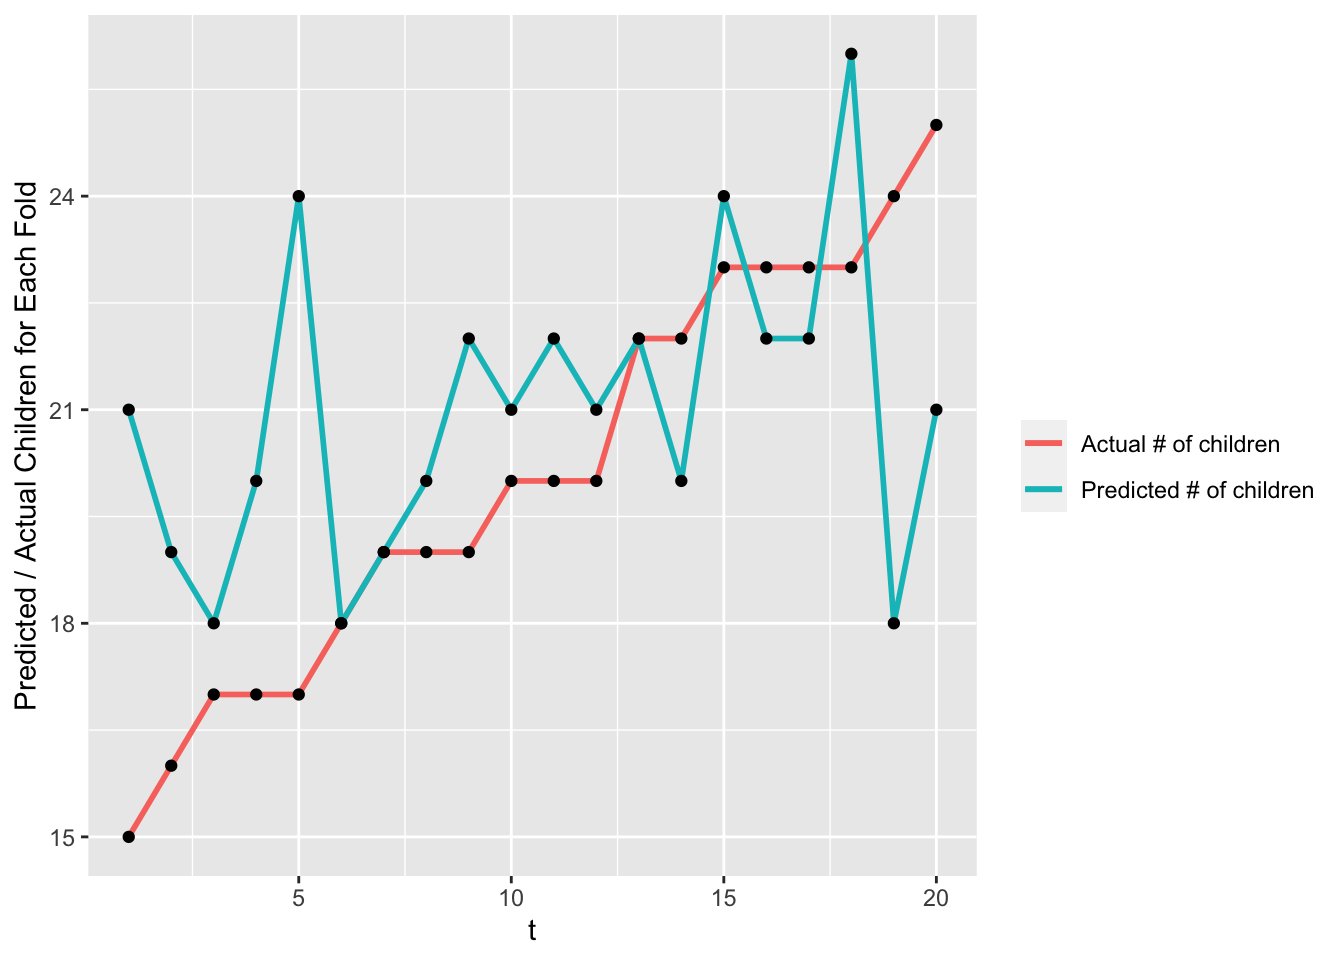
\includegraphics{Exercise2_files/figure-latex/unnamed-chunk-14-1.pdf}
\includegraphics{Exercise2_files/figure-latex/unnamed-chunk-14-2.pdf}

\hypertarget{model-validation-step-2}{%
\subsection{4.5 Model Validation: Step
2}\label{model-validation-step-2}}

\includegraphics{Exercise2_files/figure-latex/unnamed-chunk-15-1.pdf}

From the plot, the difference of each fold for actual data and predicted
model is small, which is almost smaller than 5. Therefore, our model do
well at predicting the total number of bookings with children in a group
of 250 bookings.

\end{document}
